% Main file for the GREIT Algorithm
% $Id$
\documentclass[12pt]{iopart}
\usepackage{graphicx}
%\usepackage{amsfonts}
%\usepackage{amsmath}
\newcommand{\mathbb}{\mathbf}
\newcommand{\vB}{\mbox{$\mathbf{v}$}}
\newcommand{\xB}{\mbox{$\mathbf{x}$}}
\newcommand{\xH}{\mbox{$\mathbf{\hat x}$}}
\newcommand{\nB}{\mbox{$\mathbf{n}$}}
\newcommand{\yB}{\mbox{$\mathbf{y}$}}
\newcommand{\wB}{\mbox{$\mathbf{w}$}}
\newcommand{\AB}{\mbox{$\mathbf{A}$}}
\newcommand{\BB}{\mbox{$\mathbf{B}$}}
\newcommand{\RB}{\mbox{$\mathbf{R}$}}
\newcommand{\IB}{\mbox{$\mathbf{I}$}}
\newcommand{\JB}{\mbox{$\mathbf{J}$}}
\renewcommand{\PB}{\mbox{$\mathbf{P}$}}
\newcommand{\VB}{\mbox{$\mathbf{V}$}}
\newcommand{\WB}{\mbox{$\mathbf{W}$}}
%\newcommand{\SG}{\mbox{${\boldsymbol \Sigma}$}}
\newcommand{\SG}{\mbox{${\mathbf \Sigma}$}}
\newcommand{\sG}{\mbox{${\mathbf \sigma}$}}
\newcommand{\SNR}{\mbox{\small $\mathrm{SNR }$}}
\newcommand{\NF}{\mbox{\small $\mathrm{NF }$}}
\newcommand{\EIT}{\mbox{\small $\mathit{EIT }$}}
\begin{document}

\title[GREIT: linear EIT image reconstruction]{%
GREIT: a unified approach to 2D linear EIT reconstruction of
       lung images
\\
{\small \tt DRAFT: $Date$}
}

\author{Andy Adler$^{1}$,
        John Arnold$^{2}$,
        Richard Bayford$^{3}$,
        Andrea Borsic$^{4}$,
        Brian Brown$^{5}$,
        Paul Dixon$^{6}$,
        Theo J.C. Faes$^{7}$,
        In\'ez Frerichs$^{8}$,
        Herv\'e Gagnon$^{9}$,
        Yvo G\"arber$^{10}$,
        Bart\l{}omiej Grychtol$^{11}$, 
        G\"unter Hahn$^{12}$,
        William R B Lionheart$^{13}$,
        Anjum Malik$^{14}$,
        Janet Stocks$^{15}$,
        Andrew Tizzard$^{3}$,
        Norbert Weiler$^{8}$,
        Gerhard Wolf$^{2}$%
       }

{\em {\bf TODO}: We need to clarify authors and get complete addresses}
\address{ $^{1}$Systems and Computer Engineering,
                Carleton University, Ottawa, Canada}
\address{ $^{2}$Division of Critical Care Medicine, Department of Anesthesia,
                Children's Hospital Boston, Harvard Medical School,
                Boston, MA, USA}
\address{ $^{3}$School of Health and Social Sciences,
                Middlesex University, London, UK}
\address{ $^{4}$School of Engineering, 
                Dartmouth College, Hanover, NH, USA}
\address{ $^{5}$Medical Physics, University of Sheffield, UK}
\address{ $^{6}$Cardinal Health Care, London, UK}
\address{ $^{7}$Department of Physics and Medical Technology,
                V.U. university medical center, Amsterdam, Netherlands}
\address{ $^{8}$Department of Anaesthesiology and Intensive Care Medicine,
                University of Schleswig-Holstein, Kiel, Germany}
\address{ $^{9}$D\'epartement de g\'enie \'electrique,
                \'Ecole Polytechnique de Montr\'eal, Canada}
\address{$^{10}$Dr\"ager Medical, L\"ubeck, Germany}
\address{$^{11}$University of Strathclyde, Glasgow, UK}
\address{$^{12}$Department of Anaesthesiological Research,
                University of G\"ottingen, Germany}
\address{$^{13}$School of Mathematics, University of Manchester, UK}
\address{$^{14}$Maltron International, Rayleigh, UK}
\address{$^{15}$Institute of Child Health,
                University College London, UK}



\begin{abstract}
Recently, Electrical Impedance Tomography (EIT) has begun to see a
significant clinical interest for the application of monitoring
mechanically ventilated patients.
EIT has clinical promise to help better manage these patients,
because it is able to non-invasively
provide a continuous image of the distribution of ventilation. 
However, most clinical and physiological research in lung EIT
is done using older and proprietary algorithms; this is
an obstacle to interpretation of EIT data because the
reconstructed images are not well characterized.
To address this issue, we are developing a
consensus linear reconstruction algorithm for lung EIT,
called GREIT (Graz consensus Reconstruction algorithm for EIT).
This paper describes the unified approach to 
linear image reconstruction developed for GREIT,
and the tools and evaluation methodology for
clinical and experimental testing of the algorithm.
The framework for the linear reconstruction algorithm
consists of:
1) detailed finite element models of a representative
 adult and neonate thorax;
2) consensus on the performance figures of merit for
 EIT image reconstruction, which are:
a) uniform amplitude response,
b) low and uniform reconstructed position error,
c) low, uniform and circular small point spread function,
d) good noise performance,
e) low sensitivity to electrode and boundary movement,
f) low artefact amplitude on clinical and experimental data;
and
3) A systematic approach to optimize a linear reconstruction
 matrix to desired performance figures.
This approach represents the consensus of a large and representative
group of experts in EIT algorithm and clinical applications.
All software and data to implement and test GREIT has be
made available under an open source license which allows free
research and commercial use. These tools will be used in
the clinical and experimental validation stage of GREIT development.
\end{abstract}

\noindent{\it Keywords\/}:
Electrical Impedance Tomography,
Lung Function Imaging,
Image Reconstruction,

\section{Introduction}
Electrical Impedance Tomography (EIT) measures conductivity
changes within a body from current stimulation and voltage
measurement on the body surface. One of the most promising
applications of EIT is for measuring the lungs, since these
are large organs which undergo large changes in conductivity
during normal functioning. Indeed, lung function measurement
was among the first physiological applications of this technology.
(Barber and Brown 1984).
While there are several medical imaging and instrumentation
technologies to measure ventilation, EIT is unique in that it
is able to non-invasively and continuously monitor the distribution of 
ventilation. Based on these advantages, there is significant
interest in EIT to 
monitor patients with respiratory compromise.

One limitation is that most clinical and physiological research
on lung EIT is being done using proprietary variants of
older image reconstruction algorithms, such as the backprojection
algorithm as implemented
in the Sheffield (Brown and Seagar, 1987)
or G\"ottingen (Hahn \etal, 2001) EIT systems.
The algorithms, although very successful for the time,
   do not incorporate advances that have been made over the last
   20 years;
This is an obstacle to clinical use of EIT because
these algorithms have numerous specific issues, such
   as spatial non-uniformity in image amplitude, position
   and resolution which make interpretation of regional
   ventilation difficult and error prone.
One specific issue, is that 
artefacts can be incorrectly placed (ie. movement of
   the skin can appear as changes in the lung regions),
   resulting in incorrect interpretations.
Many other approaches to reconstruct EIT images have been
proposed, incorporating many advances. Such approaches
have not been widely used clinically and experimentally
because there was a lack of a agreement on which
approaches were best (and if they could be combined).

To address this issue, we are developing a
consensus linear reconstruction algorithm for lung EIT,
called GREIT (Graz consensus Reconstruction algorithm for EIT),
since early discussions took place at the 2007 ICEBI conference
in Graz, Austria (ref). Our aim is to develop a standard which
has broad agreement from experts in the mathematical,
engineering, physiological, and clinical EIT communities.
Such an approach is feasible because there is general
consensus amongst experts in EIT image processing of
the ``ingredients'' that should
be part of a robust and high performance linear algorithm
for 2D EIT of the lungs.
This paper describes the unified approach to 
linear image reconstruction developed for GREIT,
and the tools and evaluation methodology for
clinical and experimental testing of the algorithm.
The framework for the linear reconstruction algorithm
consists of:
1) detailed finite element models of a representative
 adult and neonate thorax;
2) consensus on the performance figures of merit for
 EIT image reconstruction, which are:
and
3) A systematic approach to optimize a linear reconstruction
 matrix to desired performance figures.

The current work is limited to the reconstruction algorithm.
We do not propose calibration tests, data formats or phantoms, standards
for image interpretation or EIT based lung parameters; 
we do not feel there is sufficient experience yet to reach
consensus in these areas.
It is important to clarify that there is no financial
goal to the development of this algorithm.
All developed algorithms, software
models and simulation and experimental test data used
in this algorithm have been
made available under an open source license as part of
the open source EIDORS distribution (Adler and Lionheart, 2006);
this license permits
royalty free use in both research and commercial applications.


The goals identified for GREIT are for:
\begin{itemize}
\item
 single and double ring electrode
configurations with Sheffield-type EIT systems, using
      adjacent current injection and measurement.
\item
 linear (real-time) reconstruction of a 2D conductivity
change image, based on a 3D forward model
\item
 quantitative reconstructions:
   given an input in transfer impedance ($\Omega$) units,
                    the output is in impedivity change ($\Omega\cdot m$)
\item
 settings for all parameters:
     any tunable parameters must have assigned
     values in the recommended algorithm.
\item
 published reconstruction matrices for
      a $32\times 32$ pixel array
      for a single ring of $16$, $12$ and $8$ 
      electrodes, for the shapes:
   a) neonate chests, 
   b) adult chests (for perhaps several body shapes), and 
   c) cylindrical tank phantoms.
 For other shapes and electrode configurations,
   reconstruction matrices may be calculated from the
   provided source code.
\end{itemize}

These limitations represent our opinions on the limits
to areas understood sufficiently well in the EIT community
to reach consensus. We do not propose such limits are ideal;
in fact, we activly encourage work to overcome them,
such as planar placement of electrodes and the consequent 2D images. 

\section{Methods: performance figures of merit}
\label{sec:figmerit}

In this section, we elaborate on a set of criteria which 
characterize the performance of an ideal reconstruction
algorithm. Clearly, there is an inherent tension between
the measures, such that it is not possible to 
simultaneously optimize all measures. Instead, we proceed
as follows. After establishing the performance measures,
we describe a unified methodology to calculate a reconstruction
matrix which is an optimized compromize of criteria
weighted by the consensus importance of each.  


Each algorithm will be evaluated against the
following criteria.

\subsection{Amplitude Response}
   \begin{itemize}
   \item Output amplitude is correct ($\Omega \cdot m$)
   \item the amplitude response is uniform for all radial positions.
   \end{itemize}

\subsection{Position Error}
   \begin{itemize}
   \item low average position error
   \item uniform position error with radial position
   \end{itemize}

\subsection{ Resolution}
   \begin{itemize}
   \item small average PSF size
   \item uniform PSF size with radial position
   \item no (or very little) overshoot in the PSF
  (overshoot is the negative ring around a target)
   \item circular PSF
   \end{itemize}

\subsection{ Noise Performance}
   \begin{itemize}
   \item low average noise amplification
   \end{itemize}

\subsection{ Boundary shape and electrode sensitivity}
   \begin{itemize}
   \item low sensitivity to electrode movement
   \item low sensitivity to boundary distortions
         (with breathing and posture change)
   \item low sensitivity to changes in electrode contact impedance
   \end{itemize}

\section{Methods: forward models}

Finite element models (FEM) have been developed for three
different geometries: a cylindrical phantom (useful for 
phantom studies and experimental testing), a
neonate chest and an adult chest. The primary difference
between the neonate and adult chest shapes are due to
the size of the electrodes.

\begin{figure}[bhtp]
\begin{center}
  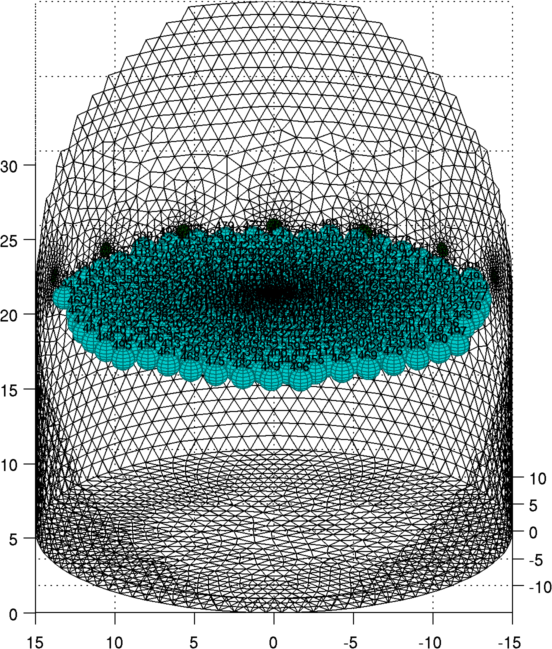
\includegraphics[width= 0.4 \textwidth, bb=0 0 444 517]
         {../../tutorial/GREIT-evaluation/simulation_3d_test02a.png}

\caption{ \label{fig:fm2}
{\em left:} FEM of the cylindrical phantom
{\em right:} FEM of the neonate chest 
}
\end{center}
\end{figure}

Issues to consider for the forward modelling are:
\begin{itemize}
\item
Electrodes placed at the intercostal space
(as per discussion on electrode placement)
\item
Refinement of FEM mesh in electrode region
\item
Size of FEM in 50k elements is adequate
\item
3D FEM models are required
\item
Use of complete electrode model (ref)
\item
It is necessary to simulate targets at various
\\ $-$ contrast levels
\\ $-$ background lung conductivity levels
\\ $-$ 3D (off plane) positioning
\item
\end{itemize}

Issues that have not been determined
\begin{itemize}
\item
Is it necessary to have separate male / female models
\item
Is it necessary to have models for different patient sizes
\item
What levels of background lung conductivity should be included
\end{itemize}


The method presented in this section is general,
applying for an arbitrary number of electrodes  with 
arbitrary placement. However, the current implementation
is designed for electrodes placed in a plane around the
chest at the level of the ???

\section{Methods: Reconstruction algorithm framework}

This section represents a framework to calculate
a linear image reconstruction matrix which is optimized
to a set of performance requirements. This approach
is based a experience with a large number of 
linear regularized EIT reconstruction approaches
(REFS??). The key difference is that this framework
is based on a set of performance requirements, whereas
previous reconstruction algorithms are based directly on
the underlying mathematical models and do not express
the performance requirements explicity.
The value of this approach is that is allows
performance requirements (established in our case
via consensus) may be directly encoded into the
reconstruction algorithm.

We consider an EIT system with $n_E$ electrodes applied to a body
using sequential current stimulation with parallel voltage
measurement. Using these electrodes, $n_E$ current stimulation
patterns are sequentially applied and $n_V$ differential
measurements are made for each stimulation.  For an adjacent drive
EIT system, voltages are typically not measured at driven
electrodes, and $n_V = n_E - 3$.  Each data frame measures
a vector, $\vB\in\mathbb{R}^{n_M}$, of $n_M= n_E n_V$ data points
(some of which are redundant if the medium is not changing).
Difference EIT calculates difference data $\yB$, ($[\yB]_i =
[\vB_2]_i - [\vB_1]_i$; or the normalized difference data $[\yB]_i
= ([\vB_2]_i - [\vB_1]_i)/[\vB_1]_i)$. To improve its precision,
$\vB_1$ is typically averaged over many data frames, at a time
when the conductivity distribution may be assumed to be stable;
 we thus assume that $\vB_1$ is noise free.

The body under investigation is modelled using a finite element
model (FEM) which discretizes the conductivity onto $n_N$
piecewise smooth elements, represented by a vector
$\sG\in\mathbb{R}^{n_N}$ (In this paragraph, $\sG$ represents
conductivity; elsewhere in this paper, $\sigma$ is the standard
deviation). Again, difference EIT calculates a vector of
conductivity change, $\xB = \sG_2 - \sG_1$ between the present
conductivity distribution, $\sG_2$, and that at the reference
measurement, $\sG_1$.

\subsection{One step linear Gauss-Newton solvers}

One-step Gauss-Newton (GN) EIT reconstruction approaches have been
widely used in EIT since the late 1980's (Yorkey et al 1987,
Cheney et al 1990).
They allow use of sophisticated regularized models
of the EIT inverse problem, are able to represent this
solution as a linear reconstruction matrix, which can then allow
rapid, real-time imaging.
For small variations around the reference
conductivity $\sG_1$, the relationship between $\xB$ and $\yB$ can
be linearized (giving the difference EIT forward model):
\begin{equation}\label{FM}
\yB=\JB\xB+\nB
\end{equation}
where
$\JB\in\mathbb{R}^{n_M\times n_N}$ is the Jacobian or sensitivity
matrix and $\nB\in\mathbb{R}^{n_M}$ is the measurement noise which is
assumed to be uncorrelated white Gaussian. $\JB$ is calculated from
the FEM as
$\JB_{ij}=\left.
     \frac{\partial\yB_i}{\partial\xB_j}
          \right|_{\sG_1}$,
and depends on the FEM, current injection patterns, the reference
conductivity, and the electrode models. This system is
underdetermined since $n_N > n_M$. 
Regularization techniques are requied
in order to calculate a conductivity change
estimate, $\xH$, which is both
faithful to the measurements, $\yB$, and to
{\em a priori} constraints on a ``reasonable'' image.

The GN inverse problem seeks to
calculate a solution, $\xH$, to the EIT inverse problem
in terms of a generalized Tikhonov regularization 
expressed as the minimum of a sum of quadratic norms
\begin{equation}\label{IM}
 \|\yB-\JB\xH\|_{\Sigma_n^{-1}}^2 +
 \|\xB-\xB^\circ\|_{\Sigma_x^{-1}}^2
\end{equation}
where $\xB^\circ$ represents the expected value of element
conductivity changes, which is zero for  difference EIT.
$\SG_n\in\mathbb{R}^{n_M\times n_M}$ is
 the covariance matrix of the measurement noise $\nB$. Since
$\nB$ is uncorrelated, $\SG_n$ is a diagonal matrix with
$[\SG_n]_{i,i}=\sigma_i^2$, where $\sigma_i^2$ is the noise variance at
measurement $i$. $\SG_x\in\mathbb{R}^{n_N\times
n_N}$ is the expected image covariance.

It is worth noting that many other regularized approaches
to EIT have been used, such as the
TSVD (truncated singular valud decomposition, REFS),
and
SIRT (simultaneous iterative reconstruction technique, REFS).
All linear approaches are structurally similar; however
the formulation in (\ref{IM}) is more general
as it explicitly exposes the selection of image reconstruction
parameters.



Typically,  covariance matrices
$\SG_n$ and $\SG_x$ are not calculated directly, but
are modelled heuristically from {\em a priori}
considerations as 
 $\VB = \sigma_n^{2}\SG_n$
 and
 $\PB = \sigma_x^{2}\SG_x$,
where $\sigma_n$ is the average measurement noise amplitude and
$\sigma_x$ is the {\em a priori} amplitude of conductivity change.
$\VB$ models the measurement accuracy. For uncorrelated noise,
each diagonal element is proportional to the signal to noise
ratio. For difference EIT with identical channels, $\WB=\IB$. The
regularization matrix $\VB$ may be understood to model the
likelihood of image elements and their interactions.

By solving (\ref{IM}), a linearized, one-step inverse solution is
obtained as
\begin{eqnarray}\label{GN_solution}
\xH&=&\left(
    \JB^T \frac{\VB^{-1}}{\sigma_n^2} \JB 
     +
    \frac{\PB^{-1}}{\sigma_x^2} 
    \right)^{-1}
    \JB^T \frac{\VB^{-1}}{\sigma_n^2}\yB
\nonumber \\
   &=&\left(
    \JB^T \VB^{-1} \JB + \lambda^2 \PB^{-1}
    \right)^{-1}
    \JB^T \VB^{-1} \yB
\end{eqnarray}
where parameter  $\lambda=\sigma_n/\sigma_x$ is
often called the ``regularization hyperparameter'' and
controls the trade-off
between resolution and noise attenuation in the reconstructed
image.
The matrix,
$\RB=\left(\JB^T\BB^{-1}\JB+\lambda^2\PB^{-1}\right)^{-1}\JB^T\VB^{-1}$
is the linear, one-step inverse.
In (\ref{GN_solution}), the term in the inverse is of size
$n_N\times n_N$. To save computational time, and improve inverse
accuracy and stability, matrix $\RB$ may be rewritten using
using the {\em data form}, or {\em Wiener filtering form} as:
\begin{equation}\label{opti_sol}
 \RB =\PB\JB^T
    \left(
       \JB\PB\JB^T+\lambda^2\VB
   \right)^{-1}
\end{equation}
Using (\ref{opti_sol}), the size of the term in the inverse is
reduced to $n_M\times n_M$.

If image elements are assumed to be independent with identical
expected magnitude, $\PB$ becomes an identity matrix $\IB$ and
(\ref{GN_solution}) uses zeroth-order Tikhonov regularization. For
EIT, such solutions tend to push reconstructed noise toward the
boundary, since the measured data are much more sensitive to
boundary image elements. Instead, $\PB$ may be scaled with the
sensitivity of each element, so that each diagonal element $i$ 
$[\PB^{-1}]_{i,i} = \left[ \JB^T \JB
\right]_{i,i}^p$. This is the NOSER prior of Cheney et al (1990)
for an exponent $p=1$. Many other prior matrices have been
proposed: to model image smoothness as a penalty for non-smooth
image regions, $\PB$ may be set to the discrete Laplacian filter
(Vauhkonen, 1998b), a discrete high pass Gaussian filter (Adler
and Guardo, 1996), or based on variance uniformization
constraints (Cohen-Bacrie et al 1997).

In this paper, the NOSER prior is used for calculating the matrix
$\PB$ with $p=0.5$.
Because it is diagonal, $\PB$ can be
inverted without numerical difficulties. The choice of exponent is
a heuristic compromise between the pushing noise to the boundary
($p=0$) or to the centre ($p=1$).


\subsection{GREIT image reconstruction approach}

 from a FEM of imaged subject and an estimate of
the noise level in the EIT data.
Given a set of input data $\yB_k$ ($M\times1$) which 
represent:
1) simulated conductivity change,
2) noise,
3) boundary movement,
and
4) conductivity change outside the plane of interest.

We define a set of desired images $\xH_k$ ($N\times1$),
and data weightings $\wB_k$ ($M\times1$), and an associated
diagonal weighting matrix $WB_k$, such that 
$\wB_k = diag(\WB_k)$.

The reconstruction matrix $\RB$ ($N\times M$) is a linear
map of measurements to image.
Define an error $\epsilon$ which measures the fit
of reconstructed images from each sample measurement to
the desired values
\begin{equation}
\epsilon^2 =
\sum_k \|\WB_k ( \xH_k - \RB \yB_k ) \|^p
\end{equation}
where $p$ is the error norm used; in this paper we use $p=2$
as this allows a linear formulation for $\RB$. 

{\em {\bf TODO}: add development here}

The linear fit value of $\RB$ is thus
\begin{equation}
\RB\{:\} = \BB^t (\BB \BB^t)^{-1} \AB\{:\}
\end{equation}
where the notation $\{:\}$ represents column
concatenation of a matrix, and
\begin{equation}
\AB = \sum_k \WB_k \xB_k \yB^t
\end{equation}
and $\BB$ is a vertical concatenation of $N$
($M \times M$) blocks $\BB_k$ where
\begin{equation}
\BB_i = \sum_k [\wB_k]_i \xB_k \yB^t
\end{equation}




\section{Methods: Evaluation}

Evalulation is performed in two stages. First algorithm performance
is evaluated against the figures or merit in section
\ref{sec:figmerit}.
Next, we compare to a representative set of  clinical 
and experimental data.

\subsection{Performance figure or merit}


\section{Results}

\begin{figure}[bhtp]
\begin{center}
  
\includegraphics[width= 0.2 \textwidth, bb=0 0 32 32]
         {../../tutorial/GREIT-evaluation/simulation_test_imgs/simulation_test03_1.png}
  
\includegraphics[width= 0.2 \textwidth, bb=0 0 32 32]
         {../../tutorial/GREIT-evaluation/simulation_test_imgs/simulation_test03_2.png}
  
\includegraphics[width= 0.2 \textwidth, bb=0 0 32 32]
         {../../tutorial/GREIT-evaluation/simulation_test_imgs/simulation_test03_4.png}
\caption{ \label{fig:rimage}
Reconstructed images. The conductivity target location is shown in green (the target is a circle, but shows as a small square in this image)
{\em left:} Sheffield Backprojection,
{\em center:} NOSER
{\em right:} GREIT
}
\end{center}
\end{figure}

\subsection{Experimental data}

\begin{figure}[bhtp]
\begin{center}
  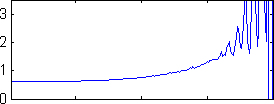
\includegraphics[width= 0.3 \textwidth, bb=0 0 280 110]
{../../tutorial/GREIT-evaluation/simulation_test_imgs/simulation_test04_11.png}
  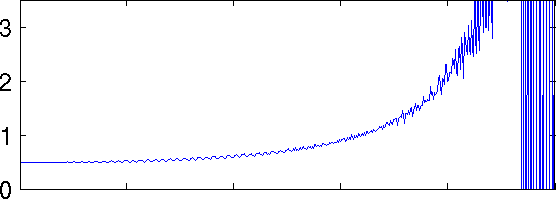
\includegraphics[width= 0.3 \textwidth, bb=0 0 280 110]
{../../tutorial/GREIT-evaluation/simulation_test_imgs/simulation_test04_21.png}
  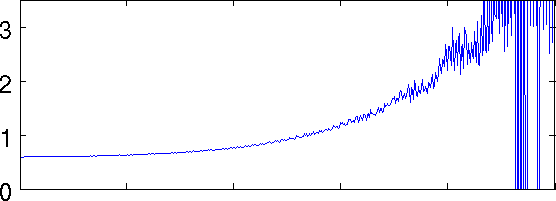
\includegraphics[width= 0.3 \textwidth, bb=0 0 280 110]
{../../tutorial/GREIT-evaluation/simulation_test_imgs/simulation_test04_41.png}
\caption{ \label{fig:rimage}
Noise Figure ({\em Want: small})                        
{\em left:} Sheffield Backprojection,
{\em center:} NOSER
{\em right:} GREIT
}
\end{center}
\end{figure}

\begin{figure}[bhtp, bb=0 0 280 110]
\begin{center}
  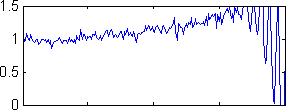
\includegraphics[width= 0.3 \textwidth, bb=0 0 280 110]
{../../tutorial/GREIT-evaluation/simulation_test_imgs/simulation_test04_12.png}
  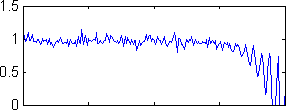
\includegraphics[width= 0.3 \textwidth, bb=0 0 280 110]
{../../tutorial/GREIT-evaluation/simulation_test_imgs/simulation_test04_22.png}
  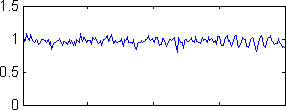
\includegraphics[width= 0.3 \textwidth, bb=0 0 280 110]
{../../tutorial/GREIT-evaluation/simulation_test_imgs/simulation_test04_42.png}
\caption{ \label{fig:rimage}
Amplitude ({\em Want: uniform})
{\em left:} Sheffield Backprojection,
{\em center:} NOSER
{\em right:} GREIT
}
\end{center}
\end{figure}

\begin{figure}[bhtp, bb=0 0 280 110]
\begin{center}
  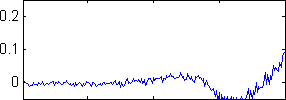
\includegraphics[width= 0.3 \textwidth, bb=0 0 280 110]
{../../tutorial/GREIT-evaluation/simulation_test_imgs/simulation_test04_13.png}
  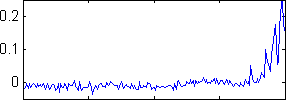
\includegraphics[width= 0.3 \textwidth, bb=0 0 280 110]
{../../tutorial/GREIT-evaluation/simulation_test_imgs/simulation_test04_23.png}
  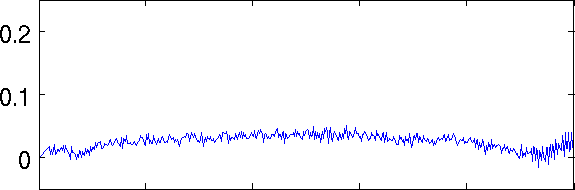
\includegraphics[width= 0.3 \textwidth, bb=0 0 280 110]
{../../tutorial/GREIT-evaluation/simulation_test_imgs/simulation_test04_43.png}
\caption{ \label{fig:rimage}
Position Error ({\em Want: small, uniform})
{\em left:} Sheffield Backprojection,
{\em center:} NOSER
{\em right:} GREIT
}
\end{center}
\end{figure}

\begin{figure}[bhtp, bb=0 0 280 110]
\begin{center}
  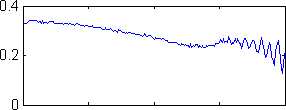
\includegraphics[width= 0.3 \textwidth, bb=0 0 280 110]
{../../tutorial/GREIT-evaluation/simulation_test_imgs/simulation_test04_14.png}
  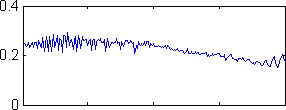
\includegraphics[width= 0.3 \textwidth, bb=0 0 280 110]
{../../tutorial/GREIT-evaluation/simulation_test_imgs/simulation_test04_24.png}
  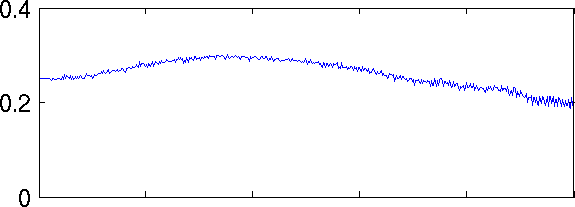
\includegraphics[width= 0.3 \textwidth, bb=0 0 280 110]
{../../tutorial/GREIT-evaluation/simulation_test_imgs/simulation_test04_44.png}
\caption{ \label{fig:rimage}
Point Spread Function ({\em Want: small, uniform })
{\em left:} Sheffield Backprojection,
{\em center:} NOSER
{\em right:} GREIT
}
\end{center}
\end{figure}

\begin{figure}[bhtp, bb=0 0 280 110]
\begin{center}
  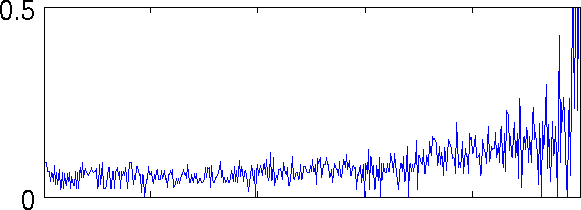
\includegraphics[width= 0.3 \textwidth, bb=0 0 280 110]
{../../tutorial/GREIT-evaluation/simulation_test_imgs/simulation_test04_15.png}
  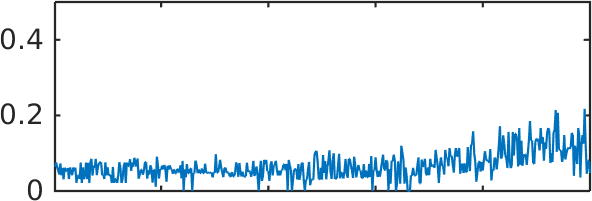
\includegraphics[width= 0.3 \textwidth, bb=0 0 280 110]
{../../tutorial/GREIT-evaluation/simulation_test_imgs/simulation_test04_25.png}
  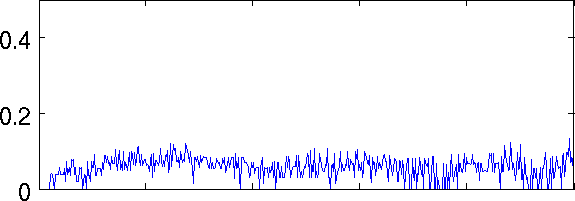
\includegraphics[width= 0.3 \textwidth, bb=0 0 280 110]
{../../tutorial/GREIT-evaluation/simulation_test_imgs/simulation_test04_45.png}
\caption{ \label{fig:rimage}
Shape Deformation ({\em Want: small, uniform})
{\em left:} Sheffield Backprojection,
{\em center:} NOSER
{\em right:} GREIT
}
\end{center}
\end{figure}

\begin{figure}[bhtp, bb=0 0 280 110]
\begin{center}
  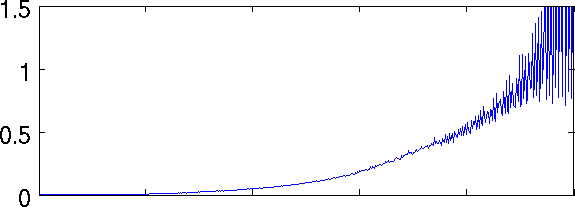
\includegraphics[width= 0.3 \textwidth, bb=0 0 280 110]
{../../tutorial/GREIT-evaluation/simulation_test_imgs/simulation_test04_16.png}
  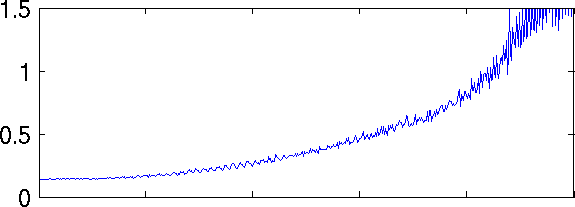
\includegraphics[width= 0.3 \textwidth, bb=0 0 280 110]
{../../tutorial/GREIT-evaluation/simulation_test_imgs/simulation_test04_26.png}
  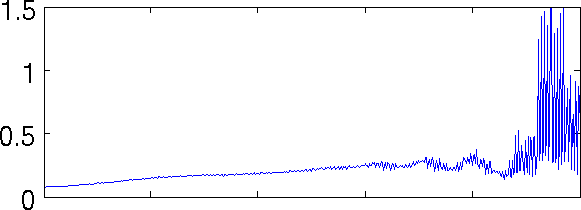
\includegraphics[width= 0.3 \textwidth, bb=0 0 280 110]
{../../tutorial/GREIT-evaluation/simulation_test_imgs/simulation_test04_46.png}
\caption{ \label{fig:rimage}
Ringing ({\em Want: small })
{\em left:} Sheffield Backprojection,
{\em center:} NOSER
{\em right:} GREIT
}
\end{center}
\end{figure}

\section{Discusion}

$-$ Summary
\\
$-$ Review of ``recipe'' for GREIT algorithm
\\
$-$ Recommended selection of parameters
\\
$-$ Discussion of remaining steps before 
    GREIT can be released.
    


\subsection{Deliverables \& Licensing}

This paper makes the following contributions. All are
available on the internet at \verb+eidors3d.sf.net/GREIT+:
All algorithms, models and test data have been made available
under an open source license which allows
gratis commercial and non-commercial use.
\begin{itemize}
\item An algorithm (described in the section ??) for reconstruction
         of EIT images
\item Software to implement this algorithm in the Matlab/GNU Octave
         language available as part of EIDORS (Adler and Lionheart, 2006)
\\
{\em License:}
    GNU LGPL (Free Software Foundation, 2007).
   This license allows
   unrestricted use and allows the provided software to
   be provided with proprietary addons. The requirement is
   that the source code of any modifications be provided to
   the users. For a commercial vendor, this requirement would
   mean that it would be possible to review and understand any
   changes made to the software.

\item Reconstruction matrices for EIT image reconstruction for
      adult and neonate chest shapes and for a cylindrical phantom.
{\em License:} Creative Commons Attribution
   License (Creative Commons, 2007). Users are permitted
   to copy to copy, distribute, transmit and adapt the work,
   under the conditions of attribution by citing this paper.

\item Experimental and Clinical data provided for evaluation of GREIT
{\em License:} Creative Commons Attribution
   License (Creative Commons, 2007). Users are permitted
   to copy to copy, distribute, transmit and adapt the work,
   under the conditions of attribution by citing the
   papers as indicated.
\end{itemize}

{\em Other items to discuss}
\\
$-$ use of $p<2$



\section*{References}

\References % Harvard style references
\item[]
Adler A and Guardo R 1996 Electrical impedance tomography:
regularized imaging and contrast detection {\em IEEE Trans. Med.
Imaging} {\bf 15} 170-179

\item[]
Adler A, Guardo R and Berthiaume Y 1996 Impedance imaging of lung
ventilation: Do we need to account for chest expansion? {\em IEEE
Trans. Biomed. Eng.} {\bf 43}(4) 414-20


\item[]
Adler A and Lionheart W R B 2006
``Uses and abuses of EIDORS: An extensible software base for EIT''
{\em Physiol Meas}
27 S25--S42

\item[]
Barber D C and Brown B H 1984
``Applied potential tomography'', 
{\em J Phys E: Sci Instrum}
 17 723--733

\item[]
Barber D C and Brown B H 1988 Errors in reconstruction of
resistivity images using a linear reconstruction technique {\em
Clin. Phys. Physiol. Meas.} 
9(suppl. A) 101--4

\item[]
Barber D C 1989
``A review of image reconstruction techniques for electrical
 impedance tomography''
{\em Med Phys}
16 162--169

\item[]
Brown B H and Seagar A D 1987 
``The Sheffield data collection system''
{\em Clin Phys Physiol Meas}
 8(Suppl A) 91--97

\item[]
Cheney M, Isaacson D, Newell J C, Simske S and Goble J C 1990
NOSER: an algorithm for solving the inverse conductivity problem
{\em Int.J.Imaging Syst.Technol.} 
2 66--75

\item[]
Cohen-Bacrie C  Goussard Y and Guardo R
1997
Regularized Re construction in Electrical
Impedance Tomography Using a Variance
Uniformization Constraint 
{\em IEEE Trans. Med. Imag.} 16 562-571

\item[]
Creative Commons/Science Commons 2007
``Creative Commons 3.0 Attribution License''
\verb+creativecommons.org/licenses/by/3.0/+

\item[]
GNU Lesser General Public License: Version 3, 29 June 2007
{\em Free Software Foundation, Inc.}
\verb+www.gnu.org/licenses/lgpl.html+

\item[]
Hahn G Thiel F Dudykevych T Frerichs I Gersing E
and Hellige G 2001
``Quantitative evaluation of the performance of
different electrical tomography devices''
{\em  Biomed Tech (Berl)}
46 91--95

\item[]
Hansen P C 1998 {\em Rank-deficient and ill-posed problems}
SIAM Philadelphia, PA, USA

\item[]
Harris N D, Suggett A J, Barber D C and Brown B H 1988 Applied
potential tomography: a new technique for monitoring pulmonary
function {\em Clin. Phys. Physiol. Meas.} {\bf 9} 79--85


\item[]
Kotre C J 1988
``A fast approximation for the calculation of potential distributions in electrical impedance tomography''
{\em Clin Phys Physiol Meas}
9 353--361

\item[]
Lionheart W, Polydorides N and Borsic A 2005 Why is EIT so hard,
in {\em Electrical impedance tomography: methods, history and
applications}, Holder D S, Ed. Bristol and Philadelphia, IOP, pp.
3-4

\item[]
McArdle F J, Suggett A J, Brown B H, and Barber D C 1988 An
assessment of dynamic images by applied potential tomography for
monitoring pulmonary perfusion {\em Clin. Phys. Physiol. Meas.}
{\bf 9}, 87-91


\item[]
Polydorides N and Lionheart W R B 2002 A Matlab toolkit for
three-dimensional electrical impedance tomography: A contribution
to the Electrical Impedance and Diffuse Optical Reconstruction
Software project {\em Meas. Sci. Technol.} {\bf 13} 1871-83


\item[]
Soleimani M, Gomez-Laberge C and Adler A 2006 Imaging of
conductivity changes and electrode movement in EIT \PM {\bf 27}
S103--S13

\item[]
Vauhkonen M, Vad\`asz D, Karjalainen P A, Somersalo E and
Kaipio J P 1998
 Tikhonov regularization and prior information in
electrical impedance tomography
 {\em IEEE Trans Med Imaging}
17 285--93

\item[]
Yorkey T J, Webster J G and Tompkins W J 1987
Comparing reconstruction algorithms for electrical
impedance tomography
{\em IEEE Trans. Biomed. Eng}
34 843--52

\item[]
Zhang J and Patterson R P 2005 EIT images of ventilation: what
contributes to the resistivity changes? \PM {\bf 26} S81--S92

\endrefs

\end{document}
